\documentclass[a4paper, 12pt]{article}
\usepackage{parskip}
\usepackage{graphicx}

\makeatletter
\def\@seccntformat#1{%
  \expandafter\ifx\csname c@#1\endcsname\c@section\else
  \csname the#1\endcsname\quad
  \fi}
\makeatother

\title{Physics Notes}
\date{}
\begin{document}

\maketitle

\section{Particles}

\subsection{The Atom}

\subsubsection{Classification}

There are two main groups of particles: Hadrons and Leptons.

Hadrons feel the strong force and are made up of quarks. The proton is the only stable baryon, while a neutron left on it's own will decay with a half life of about 11 minutes.

Leptons are fundamental particles like quarks, and do not feel the strong force. They mostly interact through the weak interaction (or EM if charged, and gravitational force as they have mass).
Leptons have a lepton number that is always conserved in a interaction. Neutrinos are leptons and have no charge, and very little mass, so they are hard to detect.

Hadrons consist of two separate families of particles: Baryons and Mesons.

Baryons consist of 3 quarks of any type. Mesons are a quark - anti quark pair.

\begin{center}
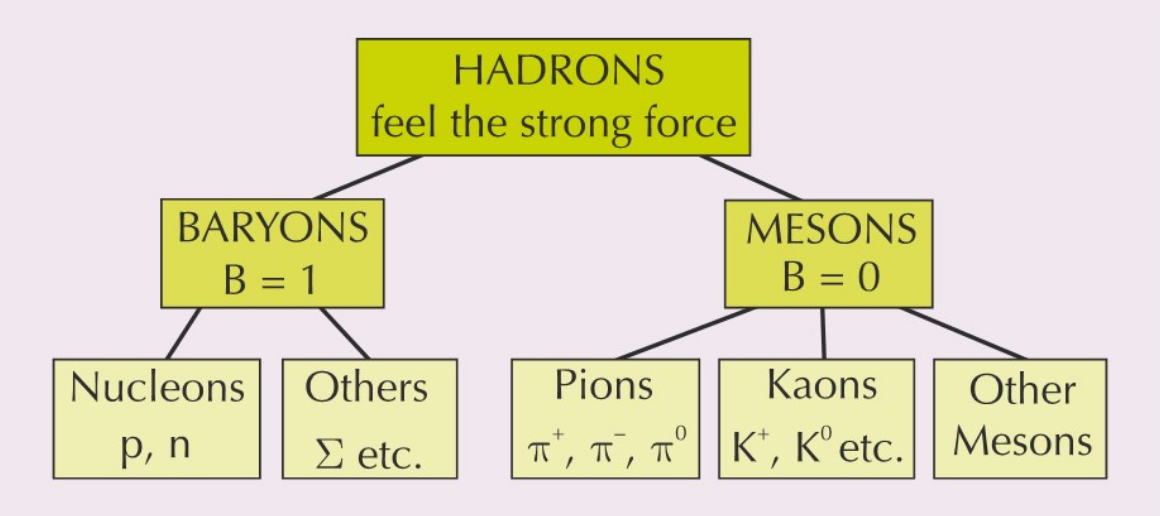
\includegraphics[height=5cm]{hadronFamily.png}
\end{center}



\subsubsection{Conservation Laws}

Conserved in all interactions:
\begin{itemize}
	\item{Baryon number}
	\item{Lepton number}
	\item{Momentum}
	\item{Charge}
\end{itemize}

Strangeness is conserved almost all interactions unless it is the weak interaction, as the weak interaction involves changing the type of a quark.

\subsubsection{Specific Mass}

Specific mass $= \frac{mass}{charge}$

\subsection{Forces}

\subsubsection{Strong Force}

The strong force binds all the nucleons in the nucleus together. It only works between hadrons.

The strong force is {\textbf{repulsive}} at distances $< 0.5$ fm, and {\textbf{attractive}} at distances $> 0.5$ fm to $3$ fm.

The strong force in the nucleus has to be stronger overall (hence the name) than the EM force to keep the nucleus together, as the protons in the nucleus are all repelling each other proton in the nucleus, where as the strong force is much more attractive for the nucleons around it, but has pretty much no effect on other nucleons.

The exchange particle for the strong force is the $\pi$ pion (a meson). (it is actually gluons but we have to say pions).


\subsubsection{Electromagnetic Force}

The electromagnetic force acts between charged particles, where $F \propto \frac{1}{r^2}$, (inverse square law) where $r$ is the distance between the centre's of the particles.

The exchange particle for the EM force is the (virtual) photon ($\gamma$), which has no mass, and travels at the speed of light ($\approx 3 \times 10^8$). It has wave-particle duality.

\subsubsection{Weak Force}

The weak force can act between any two particles. The weak force changes the flavour of a quark. This means that a strange quark can be changed into any other quark, so strangeness may not be conserved in weak interactions. It's pretty weak.

The exchange particle for the weak force is the $W^+$ or $W^-$ boson.

\subsubsection{Gravitational Force}

The gravitational force acts between all particles with mass. Like the EM force, it follows an inverse square law: $F \propto \frac{1}{r^2}$

\subsection{Decays}

Here is a graph showing the different isotopes for varying numbers of neutrons and protons, and what decay is likely to happen to each (unless stable):

\begin{center}
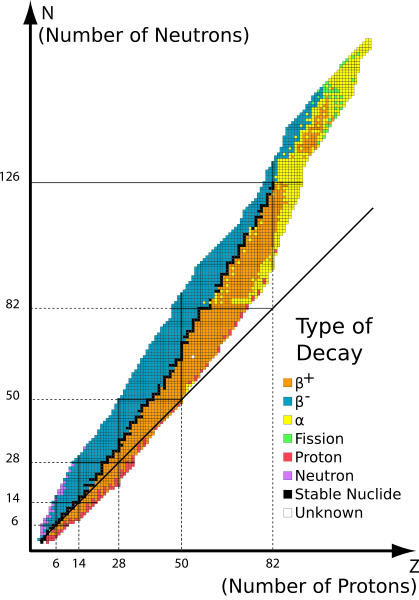
\includegraphics[height=12cm]{bandOfStability.png}
\end{center}

\subsubsection{{$\alpha$} decay}

Alpha decay is the emission of a helium nucleus from an atom's nucleus.

${\alpha^4_2}$

Alpha decay usually happens in very heavy isotopes that need to get rid of both neutrons and protons, due to the EM force in the nucleus overcoming the strong force between nucleons.

An example alpha decay would be:

$Pu^{\,240}_{\,94}\, {\Rightarrow}\, U^{\,236}_{\,92} + \alpha^4_2$

\subsubsection{{$\beta$} decay}

\textbf{$\beta^-$ decay:}

$\beta^-$ decay is when a neutron turns into a proton and electron via the weak interaction. The exchange particle is $W^-$, easy to remember since it is also negative.

Here is the equation for $\beta^-$ decay:

$n^0_1 \, \rightarrow \, p^+_1 + e^- + \overline{V_e}$

The anti neutrino $\overline{V_e}$ is to balance the lepton 

Here is the feynman diagram for $\beta^-$ decay:

\begin{center}
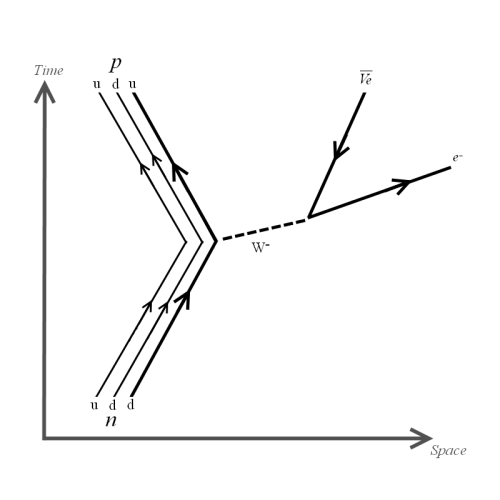
\includegraphics[height=8cm]{betaMinus.png}
\end{center}

\textbf{$\beta^+$ decay:}

$\beta^+$ decay is when a proton turns into a neutron and positron. This is key, as the position will annihilate pretty quickly with a nearby electron (as they are antiparticles), producing two high energy photons (probably gamma), so light will be emitted. The exchange particle this time is a $W^+$ boson.

Here is the equation for $\beta^+$ decay:

$p^+_1 \, \rightarrow \, n^0_1 + e^+ + V_e$

Here is the feynman diagram for $\beta^+$ decay:

\begin{center}
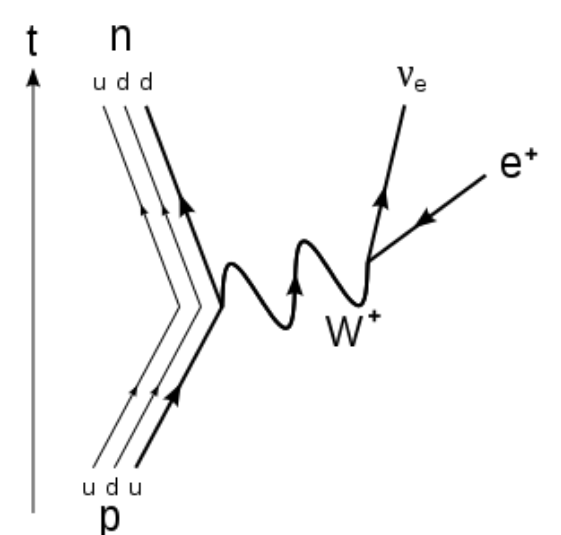
\includegraphics[height=7cm]{betaPlus.png}
\end{center}

It is pretty much the reverse of $\beta^-$.

\subsection{Electron Energy Levels}

Electrons around the nucleus can have different energy levels depending on how far away they are from the nucleus (potential energy). The further away they are from the nucleus, the less energy is required to remove the electron from that energy level and onto a higher one.

\subsection{Pair Production}

If a photon interacts with a nucleus, the energy of the photon can be converted into an electron-positron pair ($energy \rightarrow mass$). This is so that lepton number is conserved.

Here is a diagram:

\begin{center}
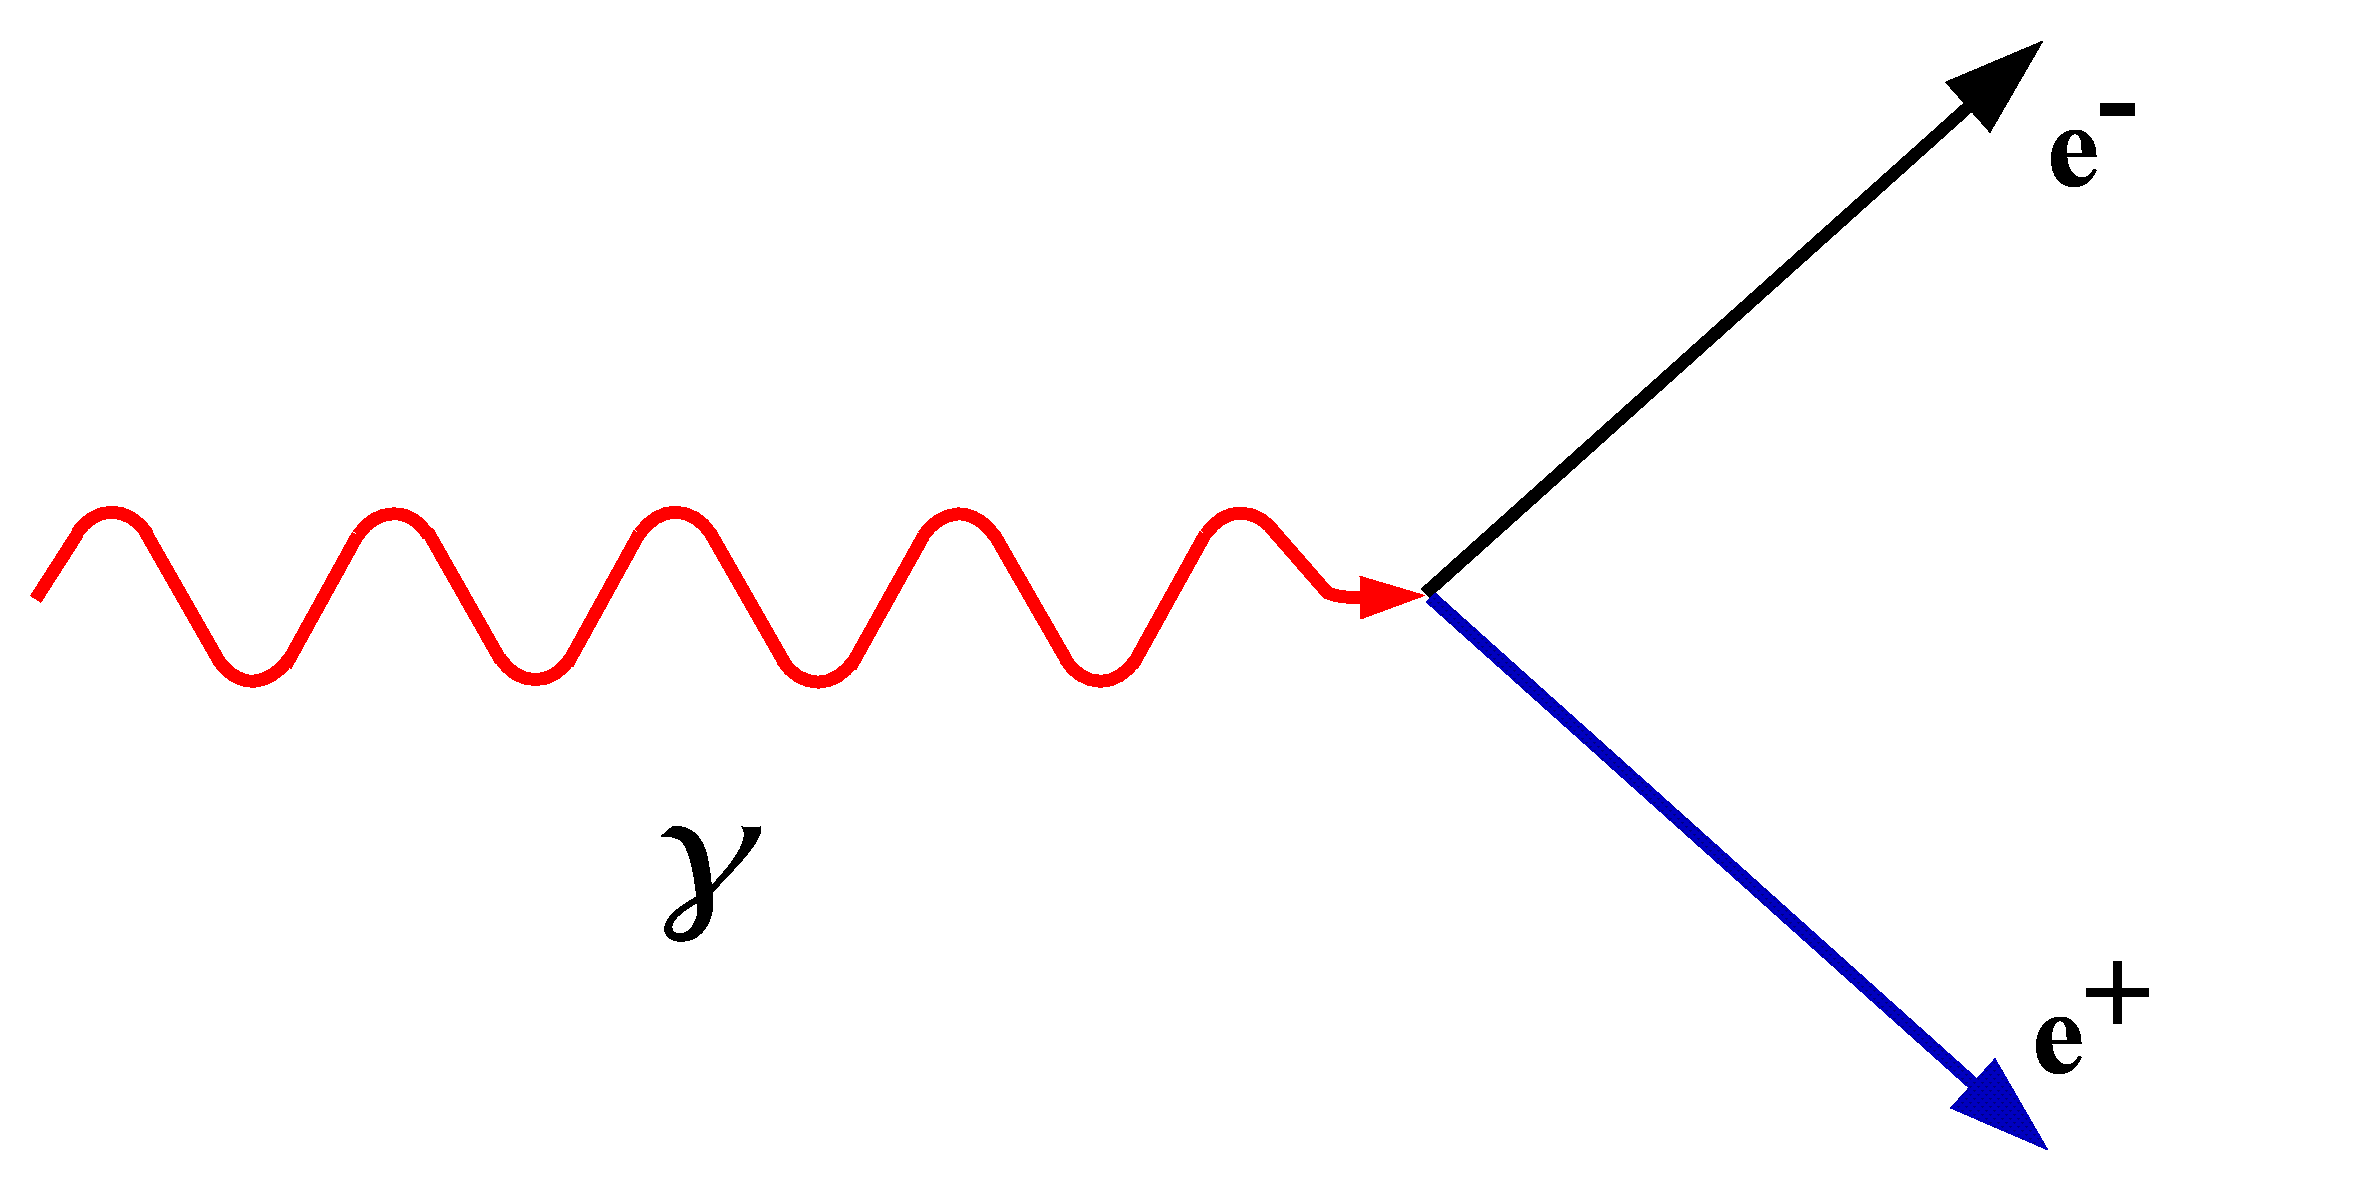
\includegraphics[height=4cm]{pairProduction.png}
\end{center}

\subsection{Electron Capture}

Electron capture is when an electron from one of the electron shells is succed into the nucleus, and interacts with a proton in the nucleus to produce a neutron and an electron neutrino. This is pretty much $\beta^+$, but there is no need for a positron since the electron at the start counteracts the charge of the proton at the start, so charge is 0 on both sides.

The equation is:

$p^+_1 + e^-_0 \, \rightarrow \, n^0_1 + Ve^0_0$

\textbf{It is important to remember that a photon will be released when the electron drops down to the ground state.}

\subsection{EM Repulsion}

When two like-charged particles get close, they repell through the EM force. \textbf{Virtual} photons are exchanged during the interaction:

\begin{center}
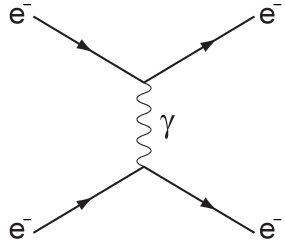
\includegraphics[height=4cm]{emRepulsion.png}
\end{center}

\end{document}
